\section{Data and Simulation Samples}
\subsection{Data}
\label{sec:subsection_data}



This analysis is based on the study of the full proton-proton collision
data from the LHC in 2012. After quality requirements, the amount 
of data used in this analysis corresponds to \lumi.
The uncertainty on the luminosity is $2.8\%$ 
following the same methodology as in \cite{Aad:2013ucp}.
%from Van-der-Meer scans taken throughout 2012.
%read this citation.
The data are selected after requiring that at least one
of a series of single lepton triggers passed during data taking, 
specifically, one of the following:
either an electron trigger 
requiring at least one isolated
electron with $\pt>24$~\GeV~, an electron trigger requiring
at least one electron 
(with no isolation requirement) with $\pt>60$~\GeV, a muon 
trigger requiring at least one isolated muon with $\pt>24$~GeV,
or a muon trigger requiring at least one muon 
(with no isolation requirement) with $\pt>36$~GeV.


\subsection{Simulation samples}
%%Do I need to talk about Monte Carlo showering, 
%%hadronization and reconstruction?
%%A general discussion of Monte Carlo could go here
MC is ...
\subsubsection{Signal Processes}
\label{sec:signal}


%%%
%If I'm going to include this, I better read up on it.
%%%
%The production \xsec without Higgs contribution has been calculated 
%to $\mathcal{O}(\alpha_s)$  corrections in Ref~\cite{Binoth:2008kt}.
%$\mathcal{O}(\alpha_s)$ corrections, Higgs boson exchange and spin 
%correlations of $W$ bosons lepton decay are also available
%~\cite{Campanario:2008yg}.  

The SM $WWW$ signal processes are implemented in the Monte
Carlo generator \vbfnlo~\cite{Arnold:2011wj,Arnold:2012xn},
which can generate partonic events at leading-order (LO) in QCD with
next-to-leading-order (NLO) cross-sections, 
and in \madgraph~\cite{MadGraph}, which can generate
partonic events at NLO  with NLO cross-sections. 
The partonic events are further processed 
by \pythiaeight~\cite{Sjostrand:2007gs} and \photos~\cite{Golonka:2005pn} 
to add effects of beam remnant interactions and initial and 
final state radiation. 
SM parameters, such as the Higgs mass,
must be provided to the MC generators as input. 
The underlying event
parameters are set in \pythiaeight~ using the ATLAS tune 
of AU2\cite{atlas:2011zja}.
The MC generators must also be provided an appropriate PDF.
The PDF used  in the LO \vbfnlo~generation is
the LO CTEQ6L1~\cite{Pumplin:2002vw} PDF set;
CT10 NLO~\cite{guzzi:2011sv}
is used in the NLO \vbfnlo~cross-section calculation.
The PDF used in the NLO \madgraph~generation 
and \xsec~calculation is CTEQ6L1 
but this is re-weighted to CT10 NLO using a k-factor of 1.08 to 1.10.
Since the MC generators are computed to finite order in perturbation
theory, renormalization and factorization scales must be chosen.
The renormalization and factorization scales are dynamically
set to the $WWW$ invariant mass in the \vbfnlo~samples; they 
are set to a fixed scale equal to the $Z$ mass in \madgraph.
The \vbfnlo~samples are restricted to leptonic decays of the $W$~bosons
where each lepton has a \pt~of at least 5~\GeV. The \madgraph~
samples include all decays of the $W$~boson, with a requirement 
that jets have a a \pt~of at least 10~\GeV~ but with no requirement
on the \pt~of leptons.
They are compared in a common fiducial phase space,
described in more detail in \sec\ref{sec:fiducial}.
The \vbfnlo~ and \madgraph~samples handle interference 
between $WH\rightarrow WWW(*)$ 
and on-shell $WWW$ production at LO, but \madgraph~is not
able to do this at NLO. As a result, the NLO \madgraph~samples
are split into sepearate samples of 
on-shell \www~ and $WH\rightarrow WWW(*)$ production.
Both sets are further split by the \www~charge mode.
For each sample, the \xsecs are summarized in \tab\ref{tab:signal_xsec} 
in their full phase space and in the common fiducial phase space.
The fiducial \xsecs are observed to be nearly the same
between the two generators.
This serves as a good check of the understanding of the 
signal process. The \madgraph~\xsecs are used throughout the 
remainder of the analysis.

%Do I need to describe the k-factors?
%It would be nice to also add some distributions from Rivet comparing
%the two at truth level.


%Describe the pdf uncertainty calculation.
%what about renormalization and factorization scales




%\begin{table}[ht]
%\centering
%\begin{tabular}{|l||c|c||}
\hline
 & \vbfnlo & \madgraph \\
\hline
\hline
Higgs mass, $m_H$ & 126.0~\GeV & \\ 
Top mass, $m_t$ & 172.4~\GeV  & \\
$Z$ mass, $m_Z$ & 91.1876~\GeV & 91.188~\GeV\\
$W$ mass, $m_W$ & 80.398~\GeV & \\
Fermi constant, $G_F$ & $1.16637\times 10^{-5}~\GeV^{-2}$ & \\
\hline
\end{tabular} 


%\caption{List of the most relevant SM parameters used as input to the 
%signal MC generation.}
%\label{tab:signal_sm_parameters}
%\end{table}


\begin{table}[ht]
\centering
\begin{tabular}{|cc||c|c|c|}
\hline
\multicolumn{2}{|c||} {Sample} &  \multicolumn{2}{c|}{Cross-section [fb]} \\
                              && Inclusive & Fiducial \\
\hline
\hline
%\multirow{3}{*}{\vbfnlo~LO} & $W^{+}W^{+}W^{-}\rightarrow l\nu l\nu l\nu$ & $3.56 \pm 0.005$ & \\
%                            & $W^{-}W^{+}W^{-}\rightarrow l\nu l\nu l\nu$ & $1.88\pm0.003$ & \\ 
%			    \cline{2-4} 
%                            & Sum & $5.44\pm0.006$ & \\ 
%\hline
\multirow{3}{*}{\vbfnlo~NLO} & $W^{+}W^{+}W^{-}\rightarrow l\nu l\nu l\nu$ & $4.95 \pm 0.007$ & $0.2050 \pm 0.0070$\\
                           & $W^{-}W^{+}W^{-}\rightarrow l\nu l\nu l\nu$ & $2.65\pm0.004$ & $0.0987 \pm 0.0037$\\ 
			    \cline{2-4} 
                           %& $WWW\rightarrow l\nu l\nu l\nu$ & $7.60\pm0.008$ & \\ 
                           & Sum & $7.60\pm0.008$ & $0.3037 \pm 0.0072$\\ 
\hline
%With PDF KFactor
\multirow{5}{*}{\madgraph~NLO} & $W^{+}W^{-}W^{+}\rightarrow \textrm{Anything}$ &$59.47\pm0.11$ & $0.0900 \pm 0.0048$\\
                        & $W^{-}W^{+}W^{-} \rightarrow \textrm{Anything}$& $28.069\pm0.076$ & $0.0476 \pm 0.0043$\\
                        & $W^{+}H\rightarrow W^{+}W^{+}W^{-}(*)\rightarrow\textrm{Anything}$ & $99.106\pm0.019$ & $0.1114 \pm 0.0029$\\
                        & $W^{-}H\rightarrow W^{-}W^{+}W^{-}(*) \rightarrow \textrm{Anything}$& $54.804\pm0.010$ & $0.0603 \pm 0.0015$\\
			\cline{2-4} 
                        & Sum & $241.47\pm0.13$ & $0.3092 \pm 0.0072$\\
%Without PDF KFactor
%\multirow{5}{*}{\madgraph~NLO} & $W^{+}W^{-}W^{+}\rightarrow \textrm{Anything}$ &$55.07\pm0.10$ & $0.0818 \pm 0.0044$\\
%                        & $W^{-}W^{+}W^{-} \rightarrow \textrm{Anything}$& $25.99\pm0.07$ & $0.0433 \pm 0.0039$\\
%                        & $W^{+}H\rightarrow W^{+}W^{+}W^{-}(*)\rightarrow\textrm{Anything}$ & $91.765\pm0.018$ & $0.1013 \pm 0.0026$\\
%                        & $W^{-}H\rightarrow W^{-}W^{+}W^{-}(*) \rightarrow \textrm{Anything}$& $50.7440\pm0.0094$ & $0.0548 \pm 0.0014$\\
%			\cline{2-4} 
%                        & Sum & $223.57\pm0.12$ & $0.2812 \pm 0.0066$\\
\hline
\end{tabular}

\caption{Inclusive and common fiducial cross-sections at NLO 
for \vbfnlo~and \madgraph~samples. 
The sum of the inclusive \xsecs are different
because of the different branching fractions in the two cases. 
The sum of the fiducial cross-sections, however, are expected to be similar because
they are computed for the same phase space, as described in \sec\ref{sec:fiducial}.
Only statistical uncertainties are shown.}
\label{tab:signal_xsec}
\end{table}


%%%%
%soud I show the dependence on scales here?
%%%%
%The dependencies of the 
%$\xsecs on the choices of scales have been studied in the two
%references~\cite{Binoth:2008kt,Campanario:2008yg}. 

% The production at LO is a pure electroweak process. The
% NLO correction brings in $\alpha_s$ which actually makes the cross
% sections more sensitive to the choices of scales. 
%It has been pointed
%out that a jet veto should reduce the scale dependence. 

%The $W$ boson is short lived, so one must study its decay products.
%As already mentioned, the focus of this analysis is on the final state 


%need to also show the MadGraph parameters
%maybe rephrase so that I can discuss both in parallel
%get generation parameters from semi-leptonic note
%report both sets of cross-sections here
%include updated info on cross-sections and PDFs 

\begin{figure}[ht!]
\centering
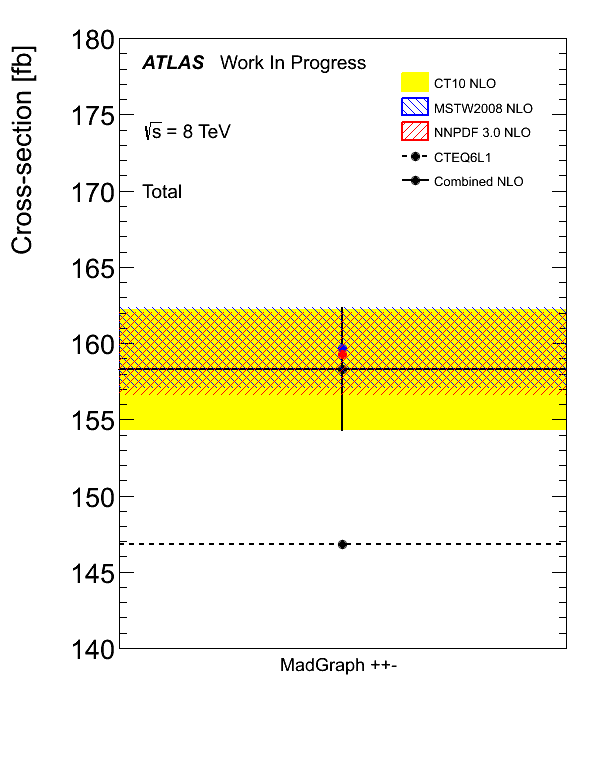
\includegraphics[width=.35\columnwidth]{figures/pdf/MADppm_total_cteq6l1.png}
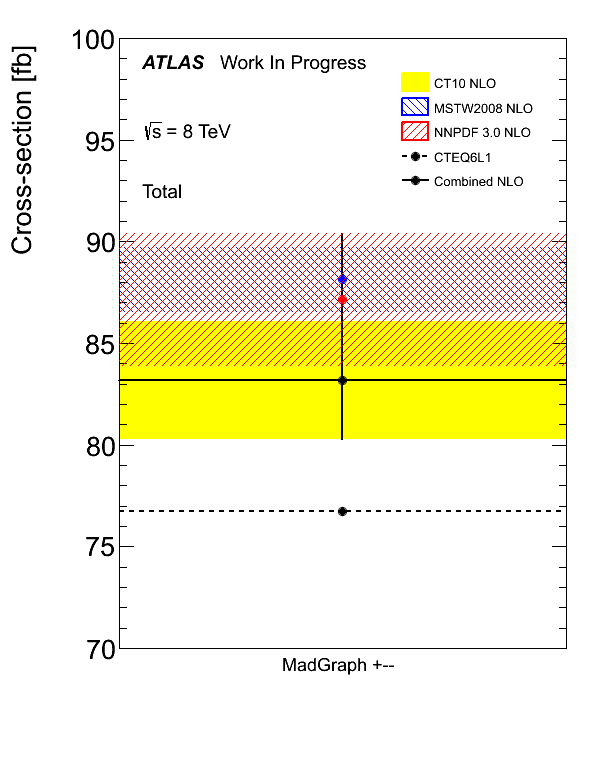
\includegraphics[width=.35\columnwidth]{figures/pdf/MADpmm_total_cteq6l1.png}
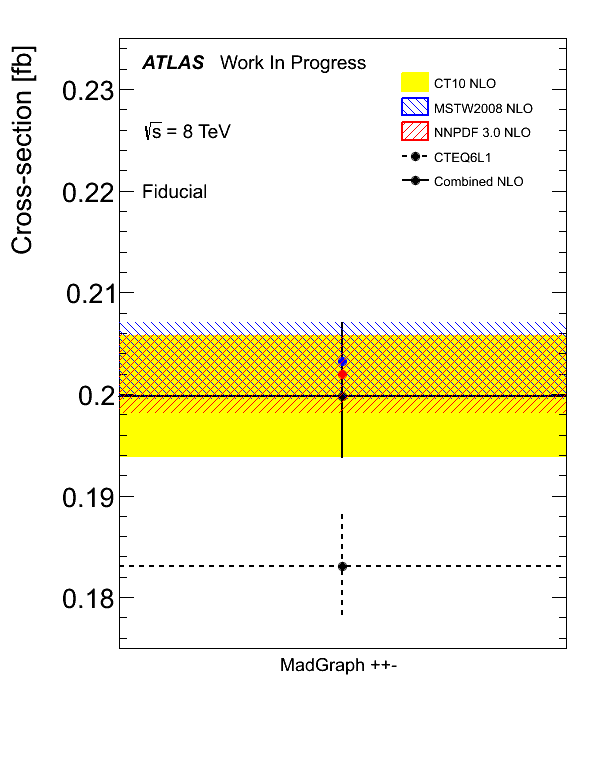
\includegraphics[width=.35\columnwidth]{figures/pdf/MADppm_fiducial_cteq6l1.png}
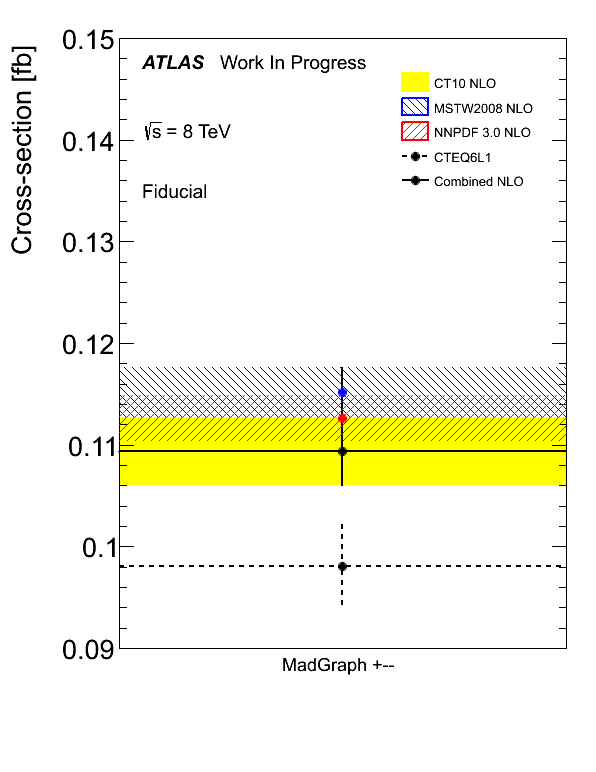
\includegraphics[width=.35\columnwidth]{figures/pdf/MADpmm_fiducial_cteq6l1.png}
\caption{The signal cross-sections for different PDFs along with their
uncertainties are shown on the {\sc MadGraph} $WWW$ signal samples
for the total $WWW$ phase space and branching fraction for
the $W^{+}W^{+}W^{-}$ (top left) and $W^{+}W^{-}W^{-}$ (top right)
charge modes
and in the fiducial region for $W^{+}W^{+}W^{-}$ (bottom left) 
and $W^{+}W^{-}W^{-}$ (bottom right).
The bands show the PDF uncertainty for CT10 NLO (solid yellow),
MSTW 2008 NLO (hashed blue), and NNPDF 3.0 NLO (hashed red). The
solid line shows the envelope of all uncertainty bands used as the final
PDF uncertainty estimate. The central value of CT10 NLO is taken as the
central value of the estimate.
The dashed-line shows the cross-section and 
statistical uncertainty for the CTEQ6L1
pdf sets used in the original generation step.}
\label{fig:signal_pdf_unc}
\end{figure}

\begin{table}[ht!]
\centering
\begin{tabular}{c|c|c}
\hline
 & \multicolumn{2}{c}{PDF Uncertainty}\\
 & $W^{+}W^{+}W^{-}$ & $W^{+}W^{-}W^{-}$ \\
\hline
\hline
Total & $+2.58\%~-2.51\%$ &  $+8.69\%~-3.47\%$ \\
Fiducial & $+3.64\%~-3.00\%$ & $+7.57\%~-3.08\%$ \\
\hline
\end{tabular}
\caption{Summary of PDF uncertainties estimated on NLO {\sc MadGraph} cross-sections
in both the fiducial and total phase space.}
\label{tab:pdfunc}
\end{table}

Uncertainties on the signal prediction mainly come from the choice of PDF, 
the inherent PDF uncertainty, and the renormalization and factorization
scales, as described in \sec\ref{sec:pdf}.
The uncertainty due to the choice of PDF is derived for the {\sc MadGraph} 
cross-sections following a modified version of the pdf4lhc
\cite{Botje:2011sn} recommendations.  The resulting 
uncertainty is shown separately for the two different charge modes
in both the fiducial and the inclusive phase
space in Table~\ref{tab:pdfunc}.
The uncertainty is determined by comparing three different PDFs:
CT10 NLO~\cite{Lai:2010vv}, MSTW2008 NLO~\cite{Martin:2009iq}, 
and NNPDF 3.0 NLO~\cite{Ball:2014uwa}. 
This comparison is presented in \fig\ref{fig:signal_pdf_unc}.  
Symmetric 68\% CL uncertainties 
are determined for CT10 NLO and MSTW 2008 NLO using the 68\% CL 
set provided for MSTW directly and the 90\%CL set for CT10 after
scaling down by 
a factor of 1.645 in order to approximate a 68 \% CL uncertainty. 
The uncertainty of the NNPDF 3.0 NLO PDF set is 
determined by using the standard deviation of the distribution 
of 101 MC PDFs provided in the PDF set; the nominal value is taken
from the mean of the same PDFs.  
The CT10 NLO PDF central value is used as the nominal 
value of the final estimate.
The final PDF uncertainty on that estimate is
taken as the envelope of the uncertainty bands for all three PDF sets.  



The uncertainty on the factorization and renormalization scales are 
determined by varying each of them independently up or down by 
a factor of two. 
The effect of these variations on the cross-sections
as compared to the nominal
are shown separately for the two different charge 
modes in \tab~\ref{tab:scaleVariation}.
The symmetric uncertainty is then determined by taking the maximum 
variation for each charge mode, 
namely, 2.62\% for $W^+W^+W^-$ and 2.53\% for $W^-W^+W^-$. 

\begin{table}[ht!]
    \centering
\begin{tabular}{cc|ccc}
\hline
& \backslashbox{$\mu_F$}{$\mu_R$}     & $\frac{1}{2}M_{WWW}$ & $M_{WWW}$ &  $2M_{WWW}$ \\
\cline{2-5}
\multirow{3}{*}{\Wp\Wp\Wm} &$\frac{1}{2}M_{WWW}$ & 2.62\% & -0.14\% & -2.11\% \\
%\cline{2-5}
&$M_{WWW}$ & 2.13\% & 0 & -2.41\% \\
%\cline{2-5}
&$2M_{WWW}$ & 1.56\% & 0.24\% & -2.42\% \\
\hline
\hline
& \backslashbox{$\mu_F$}{$\mu_R$}     & $\frac{1}{2}M_{WWW}$ & $M_{WWW}$ &  $2M_{WWW}$ \\
\cline{2-5}
\multirow{3}{*}{\Wm\Wp\Wm} &$\frac{1}{2}M_{WWW}$ & 1.91\% & 1.38\% & -2.00\% \\
%\cline{2-5}
&$M_{WWW}$ & 1.61\% & 0 & -2.53\% \\
%\cline{2-5}
&$2M_{WWW}$ & 1.25\% & -1.05\% & -2.12\% \\
\hline
\end{tabular}
\caption{The relative variation of the NLO cross sections corresponding 
to different choices of factorization and renormalization 
scales for the \Wp\Wp\Wm and \Wm\Wp\Wm  processes. }
\label{tab:scaleVariation}
\end{table}

The signal cross-sections and uncertainties are thus determined to be 
\begin{equation}
\sigma^{\textrm{Total}}_{\textrm{Theory}}= 241.47\pm0.13 ~(\textrm{Stat.}) ~^{+10.33}_{-6.08} ~(\textrm{PDF}) ~\pm 6.3 ~(\textrm{Scale}) ~\textrm{fb} %uncertainty?
\end{equation}
for the inclusive \xsec and
\begin{equation}
\label{eq:fiducial_theory}
\sigma^{\textrm{Fiducial}}_{\textrm{Theory}}= 309.2\pm7.2 ~(\textrm{Stat.}) ~^{+15.05}_{-8.36} ~(\textrm{PDF}) ~\pm 8.0 ~(\textrm{Scale}) ~\textrm{ab} %uncertainty?
\end{equation}
for the fiducial cross-section.


%should i include this
%The analysis considers events with three leptons ($e$ or $\mu$) in the final state. The contributions from events in which $W$ bosons decay to $\tau$'s, and the $\tau$'s sequentially decay to $e$ or $\mu$ should be included and is expected to be 40\% of total yield of the 3-lepton final state.  


\subsubsection{aQGC signal}
\label{sec:aqgc_signal}

MC samples of the aQGC signal processes described in \sec\ref{sec:eft}
have been generated using \vbfnlo at NLO in QCD.  (but don't we use LO?)
The cross-sections for the aQGC signal depend on the values
of the couplings $f_{s,0}$ and $f_{s,1}$. MC samples have 
been generated for a grid of points in the $f_{s,0}$ vs $f_{s,1}$ space
and their cross-sections are shown in \fig\ref{fig:aqgc_total_xsec_ununitarized_3l}. %histogram of cross-sections

\begin{figure}[ht!]
\centering
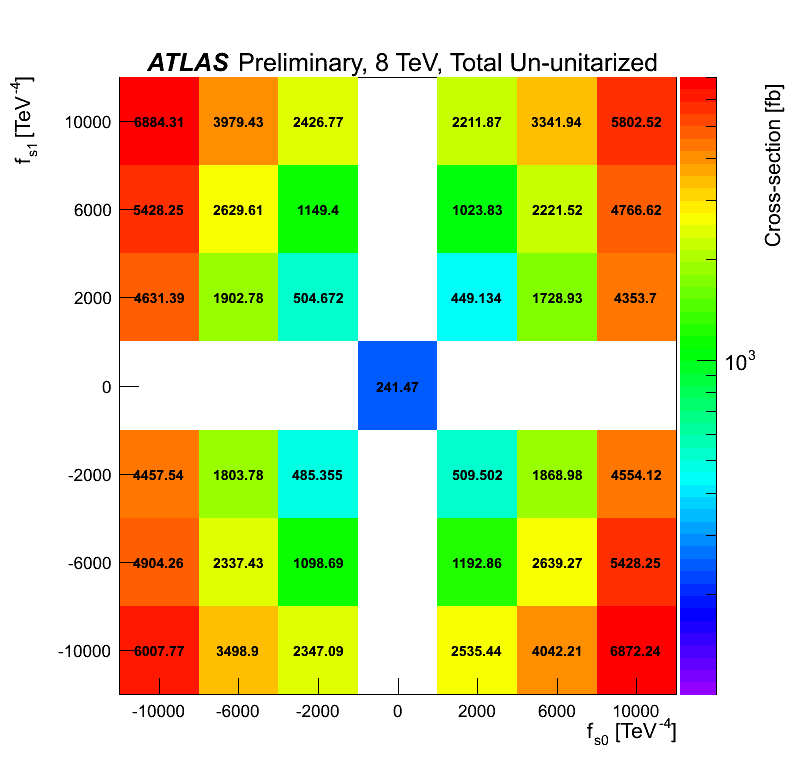
\includegraphics[width=.8\textwidth]{figures/aQGC/total_xsec/www_3l_aqgc_total_ununitarized_noratio.png}
\caption{Total cross-section for non-unitarized aQGC signal samples as a function of $f_{s,0}$ vs $f_{s,1}$.
The total SM cross-section is shown at $f_{s,0}=f_{s,1}=0$ for comparison.}
\label{fig:aqgc_total_xsec_ununitarized_3l}
\end{figure}

The issues of unitarity violation \sec\ref{sec:eft} are taken
into account using a form factor like in \eqn\eqref{eq:form_factor}.
The choices of the exponent, $n$, and form factor scale, $\Lambda$, 
are somewhat ad-hoc. Furthermore, a complete study of the unitarity
behavior of this process has never been performed, so there are not
currently detailed prescriptions on what to choose. 
However, based on discussions with the authors of \vbfnlo, who
are at the moment trying to perform these studies, an exponent
of $n=1$ is expected to be sufficient to achieve unitarity 
for this process.  As for the choice of $\Lambda$, we have
chosen to look at a few different values, which cover a wide
range but which should follow a smooth interpolation. 
This has the advantage of providing information about the
sensitivity to the form factor that can be interpreted 
by theorists as they see fit. Dedicated MC samples
are generated with the unitarization applied for values
of $\Lambda =$ 500~\GeV, 1000~\GeV, 2000~\GeV, and 3000~\GeV.
The cross-sections for each of these unitarization cases
are shown in \fig\ref{fig:aqgc_total_xsec_unitarized_3l}.

\begin{figure}[ht!]
\centering
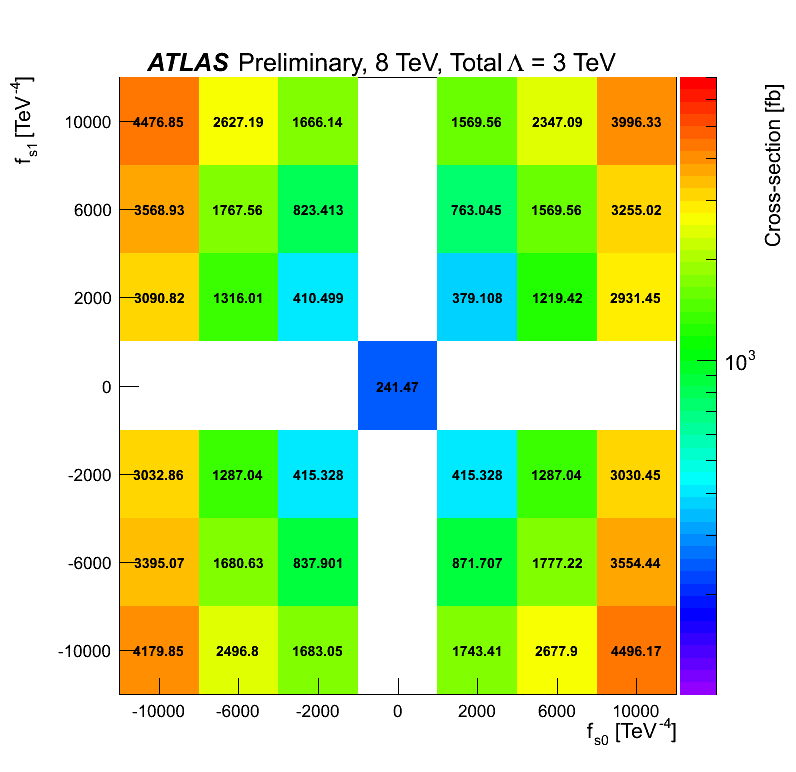
\includegraphics[width=.45\textwidth]{figures/aQGC/total_xsec/www_3l_aqgc_total_3TeV_noratio.png}
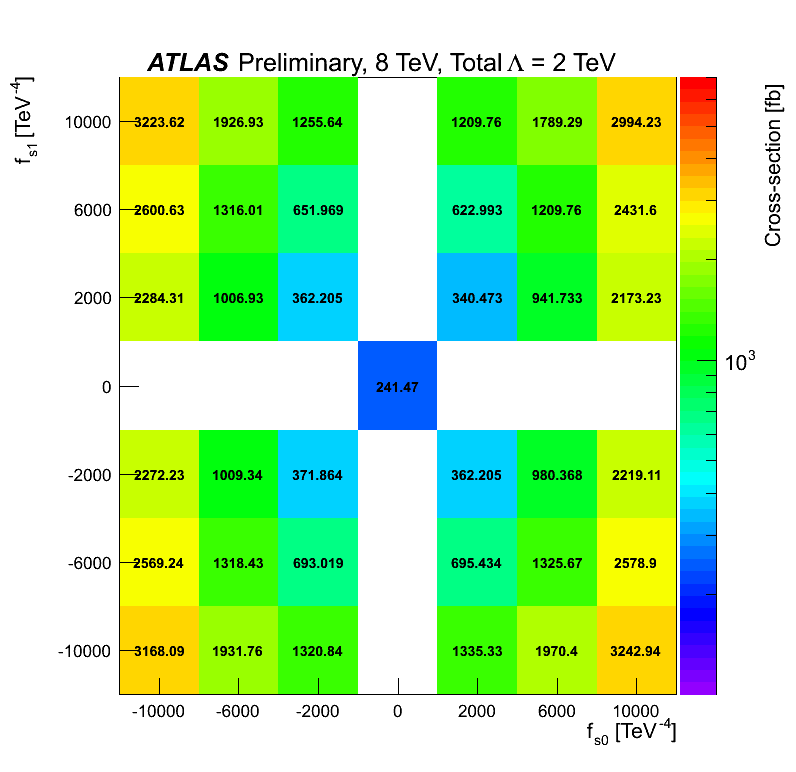
\includegraphics[width=.45\textwidth]{figures/aQGC/total_xsec/www_3l_aqgc_total_2TeV_noratio.png}
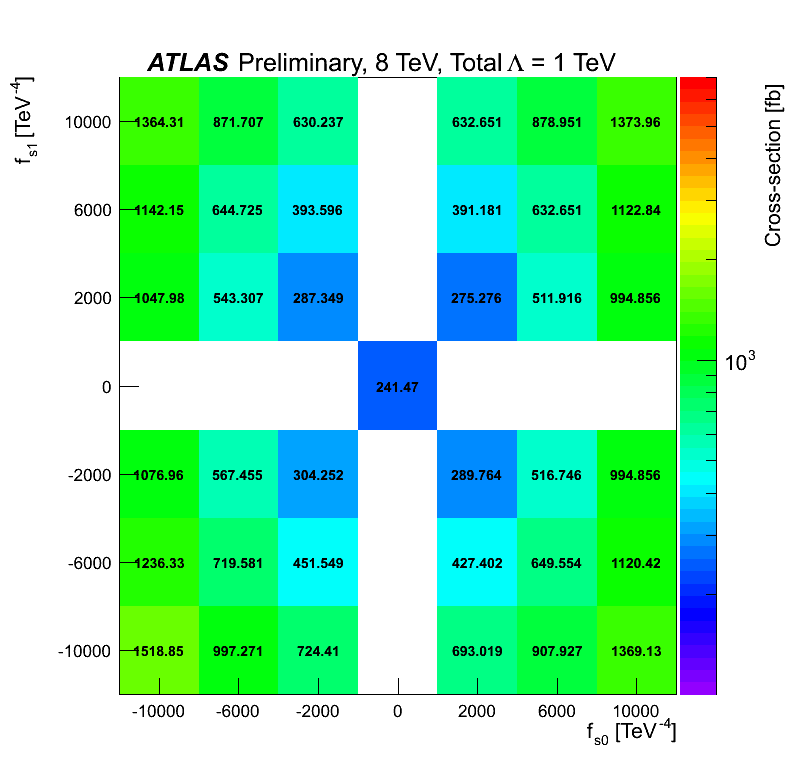
\includegraphics[width=.45\textwidth]{figures/aQGC/total_xsec/www_3l_aqgc_total_1TeV_noratio.png}
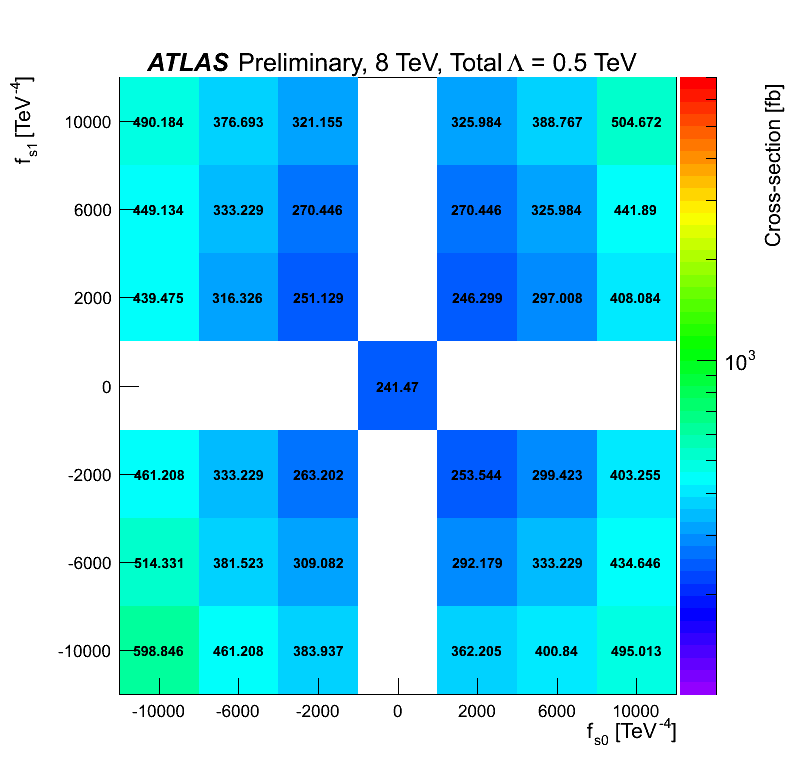
\includegraphics[width=.45\textwidth]{figures/aQGC/total_xsec/www_3l_aqgc_total_p5TeV_noratio.png}
\caption{Total cross-section for unitarized aQGC signal samples as a function of $f_{s,0}$ vs $f_{s,1}$.
Four different values of the unitarization scale, $\Lambda$, are chosen: 3~\TeV~(Top Left),
2~\TeV~(Top Right), 1~\TeV~(Bottom Left), and 0.5~\TeV~(Bottom Right).
The total SM cross-section is shown at $f_{s,0}=f_{s,1}=0$ for comparison.}
\label{fig:aqgc_total_xsec_unitarized_3l}
\end{figure}

























\subsubsection{Backgrounds samples}
\label{sec:subsection_datasets_MC}

Only processes containing 3 or more prompt
leptons ($WZ$, $ZZ$, $t\bar{t}V$, $VVV$), or 2 leptons and an 
isolated photon ($Z+\gamma$) are estimated using MC simulation 
samples in this analysis. The other processes are estimated from 
data as this will be explained in Section~\ref{sec:backgrounds_estimation}. 
The samples listed in this section and containing less than 3 prompt leptons 
have been used for preliminary or dedicated studies, but are not used for 
the determination of the final results. The MC samples are pass through the 
GEANT4~\cite{Agostinelli:2002hh} simulation~\cite{Aad:2010ah} of the ATLAS 
detector and reconstructed in the same way as the data.

The diboson and triboson samples are listed in Table~\ref{tab:sample_bkg_dibosons}. The triboson samples other than the signal, \textit{ie}: $ZWW^{*}$ and $ZZZ^{*}$ were generated using the MadGraph~\cite{Alwall_madgraph} generator, hadronized through the Pythia6~\cite{PYTHIA} parton shower, with the AUET2B~\cite{ATL-PHYS-PUB-2011-009} tunes and the CTEQ6L1~\cite{Pumplin:2002vw} PDF set. The $Z\gamma$ samples were generated with the Sherpa~\cite{sherpa} generator and the CT10~\cite{Guzzi:2011sv} PDF set. The $W\gamma$ samples were generated with the AlpGen~\cite{ALPGEN} generator, hadronized through JIMMY~\cite{Jimmy}, with the AUET2C~\cite{ATL-PHYS-PUB-2011-009} tunes and the CTEQ6L1 PDF set. Other diboson samples ($WW$, $WZ$, $ZZ$) were obtained using the Powheg~\cite{Alioli:2008gx,Nason:2004rx,Frixione:2007vw,Alioli:2010xd} generator, hadronized through the Pythia8~\cite{Sjostrand:2007gs} parton shower, with the AU2~\cite{atlasmctunes} tunes and the CT10 PDF set. Dedicated high-stat $WZ$ and $ZZ$ samples were generated to increase the statistics in all the signal region used in this analysis. They were obtained requesting the presence of 3 leptons with $\pt>7~\GeV$.

The dibosons samples where the production is due to loop induced process or Double Parton Scattering (DPS) processes are summarized in Table~\ref{tab:sample_bkg_dibosons_gg2DPI}. The loop induced processes were generated using the gg2ZZ~\cite{Binoth:2008pr} and gg2WW~\cite{Binoth:2006mf} generators, hadronized using JIMMY, with the AU2 tunes and the CT10 PDF set. The DPS processes were generated with the AU2 tunes and the CTEQ6L1 PDF set. The cross section of these processes have been evaluated for the ATLAS same sign WW analysis~\cite{Aad:2014zda}, as this will be explained in Section~\ref{sec:bkg_DPS}.

Single boson processes are summarized in Table~\ref{tab:sample_bkg_Zjets} for the $Z+$jets samples and in Table~\ref{tab:sample_bkg_wjets} for the $W+$jets samples. The $Z+$jets samples were generated with the Sherpa generator and the CT10 PDF set. Low mass Drell-Yan samples were not simluated using the GEANT4 simulation, but with the AF2 simulation, however dedicated scale factors are applied for these samples, when they are used, in the analysis. The $W+$jets samples were generated with the AlpGen generator, hadronized through JIMMY, with the AUET2C tunes and the CTEQ6L1 PDF set.

Samples containing top quarks are summarized in Table~\ref{tab:sample_bkg_top}. $t\bar{t}$ events were generated using the MCatNLO\cite{MCatNLO} generator, hadronized through JIMMY with the CT10 PDF set. Single top samples in the s-channel and in the $Wt$ channel were generated using MCatNLO hadronized through JIMMY with the CT10 PDF set. Single top samples in the t-channel were generated using AcerMC\cite{Kersevan:2004yg}, hadronized using PYTHIA6 with the AUET2B tunes and the CTEQ6L1 PDF set. Finally $t\bar{t}V$ processes were generated using the MadGraph generator, hadronized through the Pythia6 parton shower, with the AUET2B tunes and the CTEQ6L1PDF set.


 % the $Z+jets$ samples in Table~\ref{tab:sample_bkg_Zjets}, the $W+jets$ in Table~\ref{tab:sample_bkg_wjets}, and samples containing top quarks in Table~\ref{tab:sample_bkg_top}.

When $Z+$jets and $Z+\gamma$ samples are used simultaneously, an overlap removal procedure must be used to avoid double counting of FSR events. Events containing an FSR photon with $E_{T}>10~\GeV$ are explicitely vetoed out from the $Z+$jets sample. The algorithm used is the same as what was developped in the $8~\TeV$ ATLAS $WZ$ analysis~\cite{Anger:1663539}.


\begin{table}[ht!]
  \centering
  \begin{footnotesize}
\begin{tabular}{c|c|c|c|c|c|c}
\hline
    &  &  & Cross-Section &  & Event filter  \\
  Sample  & Generator & Sample type & [pb] & k-factor &  efficiency  & used in signal region\\
\hline \hline
167007 & MadGraphPythia & ZWWStar lllnulnu  &  0.0015546  &  1  &  1 & Yes \\
167008 & MadGraphPythia & ZZZStar nunullll  &  0.00033239  &  1  &  1 & Yes \\
145161 & Sherpa & eegammaPt10  &  32.26  &  1  &  1 & Yes \\
145162 & Sherpa & mumugammaPt10  &  32.317  &  1  &  1 & Yes \\
%146430 & AlpgenJimmy & Wgamma Np0 & 230.09 & 1.15 & 1 & No \\
%146431 & AlpgenJimmy & Wgamma Np1 & 59.343 & 1.15 & 1 & No \\
%146432 & AlpgenJimmy & Wgamma Np2 & 21.469 & 1.15 & 1 & No \\
%146433 & AlpgenJimmy & Wgamma Np3 & 7.1032 & 1.15 & 1 & No \\
%146434 & AlpgenJimmy & Wgamma Np4 & 2.1224 & 1.15 & 1 & No \\
%146435 & AlpgenJimmy & Wgamma Np5 & 0.46612 & 1.15 & 1 & No \\
146436 & AlpgenJimmy & Wgamma Np0 & 229.88 & 1.15 & 0.31372 & No \\
146437 & AlpgenJimmy & Wgamma Np1 & 59.518 & 1.15 & 0.44871 & No \\
146438 & AlpgenJimmy & Wgamma Np2 & 21.39  & 1.15 & 0.54461 & No \\
146439 & AlpgenJimmy & Wgamma Np3 & 7.1203 & 1.15 & 0.62974 & No \\
126928 & PowhegPythia8& WpWm ee  &  0.62  &  1.0  &  1 & No  \\
126929 & PowhegPythia8& WpWm me  &  0.62  &  1.0  &  1 & No  \\
126930 & PowhegPythia8& WpWm te  &  0.62  &  1.0  &  1 & No  \\
126931 & PowhegPythia8& WpWm em  &  0.62  &  1.0  &  1 & No \\
126932 & PowhegPythia8& WpWm mm  &  0.62  &  1.0  &  1 & No \\
126933 & PowhegPythia8& WpWm tm  &  0.62  &  1.0  &  1 & No \\
126934 & PowhegPythia8& WpWm et  &  0.62  &  1.0  &  1 & No \\
126935 & PowhegPythia8& WpWm mt  &  0.62  &  1.0  &  1 & No \\
126936 & PowhegPythia8& WpWm tt  &  0.62  &  1.0  &  1 & No \\

185813 & PowhegPythia8& ZZ 4e mll4 TriLeptonFilter & 0.07677 & 1 & 0.57204 & Yes \\
185814 & PowhegPythia8& ZZ 2e2mu mll4 TriLeptonFilter & 0.1757 & 1 & 0.49893 & Yes \\
185815 & PowhegPythia8& ZZ 2e2tau mll4 TriLeptonFilter & 0.1757 & 1 & 0.086032 & Yes \\
185816 & PowhegPythia8& ZZ 4mu mll4 TriLeptonFilter & 0.07677 & 1 & 0.58293 & Yes \\
185817 & PowhegPythia8& ZZ 2mu2tau mll4 TriLeptonFilter & 0.1757 & 1 & 0.087166 & Yes \\
185818 & PowhegPythia8& ZZ 4tau mll4 TriLeptonFilter & 0.07677 & 1 & 0.0076557 & Yes \\

181471 & Sherpa & $ZZ*\rightarrow eeee$  $m_{Z,1} > 4$~GeV, $m_{Z,2} < 4$~GeV  & 2.8286 & 0.880 & 1.0 & No \\
181472 & Sherpa & $ZZ*\rightarrow ee\mu\mu$ $m_{Z,1} > 4$~GeV, $m_{Z,2} < 4$~GeV  & 2.34503 & 0.880 & 1.0 & No \\
181473 & Sherpa & $ZZ*\rightarrow ee\tau\tau$ $m_{Z,1} > 4$~GeV, $m_{Z,2} < 4$~GeV  & 1.59326 & 0.880 & 1.0 & No \\
181474 & Sherpa & $ZZ*\rightarrow \mu\mu ee$ $m_{Z,1} > 4$~GeV, $m_{Z,2} < 4$~GeV  & 0.48613 & 0.880 & 1.0 & No \\
181475 & Sherpa & $ZZ*\rightarrow \mu\mu\mu\mu$ $m_{Z,1} > 4$~GeV, $m_{Z,2} < 4$~GeV  & 0.50835 & 0.880 & 1.0 & No \\
181476 & Sherpa & $ZZ*\rightarrow \mu\mu\tau\tau$ $m_{Z,1} > 4$~GeV, $m_{Z,2} < 4$~GeV  & 0.42288 & 0.880 & 1.0 & No \\
181477 & Sherpa & $ZZ*\rightarrow \tau\tau ee$ $m_{Z,1} > 4$~GeV, $m_{Z,2} < 4$~GeV  & 0.00403 & 0.880 & 1.0 & No \\
181478 & Sherpa & $ZZ*\rightarrow \tau\tau\mu\mu$ $m_{Z,1} > 4$~GeV, $m_{Z,2} < 4$~GeV  & 0.00401 & 0.880 & 1.0 & No \\
181479 & Sherpa & $ZZ*\rightarrow \tau\tau\tau\tau$ $m_{Z,1} > 4$~GeV, $m_{Z,2} < 4$~GeV  & 0.00411 & 0.880 & 1.0 & No \\


% 126937 & PowhegPythia8& ZZ 4e mll4 2pt5  &  0.0735  &  1.0  &  0.90765 \\
% 126938 & PowhegPythia8& ZZ 2e2mu mll4 2pt5  &  0.1708  &  1.0  &  0.82724 \\
% 126939 & PowhegPythia8& ZZ 2e2tau mll4 2pt5  &  0.1708  &  1.0  &  0.58278 \\
% 126940 & PowhegPythia8& ZZ 4mu mll4 2pt5  &  0.0735  &  1.0  &  0.91241 \\
% 126941 & PowhegPythia8& ZZ 2mu2tau mll4 2pt5  &  0.1708  &  1.0  &  0.58725 \\
% 126942 & PowhegPythia8& ZZ 4tau mll4 2pt5  &  0.0735  &  1.0  &  0.10604 \\
126949 & PowhegPythia8& ZZllnunu ee mll4  &  0.168  &  1  &  1 & No \\
126950 & PowhegPythia8& ZZllnunu mm mll4  &  0.168  &  1  &  1 & No \\
126951 & PowhegPythia8& ZZllnunu tt mll4  &  0.168  &  1  &  1 & No \\
185795  &  PowhegPythia8 &  WmZ 3e mll0p25 TriLeptonFilter  &  0.9655  &  1  &  0.051928 & Yes \\
185796  &  PowhegPythia8 &  WmZ e2mu mll0p4614 TriLeptonFilter  &  0.6326  &  1  &  0.073874  & Yes \\
185797  &  PowhegPythia8 &  WmZ e2tau mll3p804 TriLeptonFilter  &  0.1125  &  1  &  0.012544  & Yes \\
185798  &  PowhegPythia8 &  WmZ mu2e mll0p25 TriLeptonFilter  &  0.9687  &  1  &  0.054302  & Yes \\
185799  &  PowhegPythia8 &  WmZ 3mu mll0p4614 TriLeptonFilter  &  0.6479  &  1  &  0.071268  & Yes \\
185800  &  PowhegPythia8 &  WmZ mu2tau mll3p804 TriLeptonFilter  &  0.1125  &  1  &  0.01258  & Yes \\
185801  &  PowhegPythia8 &  WmZ tau2e mll0p25 TriLeptonFilter  &  0.9687  &  1  &  0.012075  & Yes \\
185802  &  PowhegPythia8 &  WmZ tau2mu mll0p4614 TriLeptonFilter  &  0.6326  &  1  &  0.01664 & Yes \\
185803  &  PowhegPythia8 &  WmZ 3tau mll3p804 TriLeptonFilter  &  0.1108  &  1  &  0.0034037  & Yes \\
185804  &  PowhegPythia8 &  WpZ 3e mll0p25 TriLeptonFilter  &  1.416  &  1  &  0.053051 & Yes  \\
185805  &  PowhegPythia8 &  WpZ e2mu mll0p4614 TriLeptonFilter  &  0.9421  &  1  &  0.075904  & Yes \\
185806  &  PowhegPythia8 &  WpZ e2tau mll3p804 TriLeptonFilter  &  0.1755  &  1  &  0.013867 & Yes  \\
185807  &  PowhegPythia8 &  WpZ mu2e mll0p25 TriLeptonFilter  &  1.412  &  1  &  0.055296 & Yes  \\
185808  &  PowhegPythia8 &  WpZ 3mu mll0p4614 TriLeptonFilter  &  0.9572  &  1  &  0.073362 & Yes  \\
185809  &  PowhegPythia8 &  WpZ mu2tau mll3p804 TriLeptonFilter  &  0.1755  &  1  &  0.013891 & Yes \\
185810  &  PowhegPythia8 &  WpZ tau2e mll0p25 TriLeptonFilter  &  1.412  &  1  &  0.012105 & Yes  \\
185811  &  PowhegPythia8 &  WpZ tau2mu mll0p4614 TriLeptonFilter  &  0.9421  &  1  &  0.016718 & Yes  \\
185812  &  PowhegPythia8 &  WpZ 3tau mll3p804 TriLeptonFilter  &  0.172  &  1  &  0.0036427 & Yes  \\
% 129477 & PowhegPythia8& WZ Wm11Z11 mll0p250d0 2LeptonFilter5  &  1.407  &  1.0  &  0.29456 \\
% 129478 & PowhegPythia8& WZ Wm11Z13 mll0p4614d0 2LeptonFilter5  &  0.9382  &  1.0  &  0.35211 \\
% 129479 & PowhegPythia8& WZ Wm11Z15 mll3p804d0 2LeptonFilter5  &  0.1746  &  1.0  &  0.16682 \\
% 129480 & PowhegPythia8& WZ Wm13Z11 mll0p250d0 2LeptonFilter5  &  1.399  &  1.0  &  0.29351 \\
% 129481 & PowhegPythia8& WZ Wm13Z13 mll0p4614d0 2LeptonFilter5  &  0.9537  &  1.0  &  0.35132 \\
% 129482 & PowhegPythia8& WZ Wm13Z15 mll3p804d0 2LeptonFilter5  &  0.1746  &  1.0  &  0.16863 \\
% 129483 & PowhegPythia8& WZ Wm15Z11 mll0p250d0 2LeptonFilter5  &  1.399  &  1.0  &  0.14289 \\
% 129484 & PowhegPythia8& WZ Wm15Z13 mll0p4614d0 2LeptonFilter5  &  0.9382  &  1.0  &  0.18256 \\
% 129485 & PowhegPythia8& WZ Wm15Z15 mll3p804d0 2LeptonFilter5  &  0.1719  &  1.0  &  0.058517 \\
% 129486 & PowhegPythia8& WZ W11Z11 mll0p250d0 2LeptonFilter5  &  0.9795  &  1.0  &  0.29694 \\
% 129487 & PowhegPythia8& WZ W11Z13 mll0p4614d0 2LeptonFilter5  &  0.639  &  1.0  &  0.35302 \\
% 129488 & PowhegPythia8& WZ W11Z15 mll3p804d0 2LeptonFilter5  &  0.1125  &  1.0  &  0.15969 \\
% 129489 & PowhegPythia8& WZ W13Z11 mll0p250d0 2LeptonFilter5  &  0.9359  &  1.0  &  0.29766 \\
% 129490 & PowhegPythia8& WZ W13Z13 mll0p4614d0 2LeptonFilter5  &  0.6488  &  1.0  &  0.35414 \\
% 129491 & PowhegPythia8& WZ W13Z15 mll3p804d0 2LeptonFilter5  &  0.1125  &  1.0  &  0.16023 \\
% 129492 & PowhegPythia8& WZ W15Z11 mll0p250d0 2LeptonFilter5  &  0.9359  &  1.0  &  0.14803 \\
% 129493 & PowhegPythia8& WZ W15Z13 mll0p4614d0 2LeptonFilter5  &  0.639  &  1.0  &  0.18657 \\
% 129494 & PowhegPythia8& WZ W15Z15 mll3p804d0 2LeptonFilter5  &  0.1107  &  1.0  &  0.056651 \\
\hline 
\end{tabular}
\end{footnotesize}
\caption{List of diboson samples used in the analysis. 
For the three lepton signal regions, it is indicated for each
sample whether or not the sample is used.  If not, it is replaced
by a data-driven fake estimate described in Section~\ref{sec:fakebg}.
All samples are used in dilepton control regions.
}
\label{tab:sample_bkg_dibosons}
\end{table}


\begin{table}[ht!]
  \centering
  \begin{footnotesize}
\begin{tabular}{c|c|c|c|c|c|c}
\hline
    &  &  & Cross-Section &  & Event filter  \\
  Sample  & Generator & Sample type & [pb] & k-factor &  efficiency  & used in signal region\\
\hline \hline
116600 & gg2ZZJimmy & ZZ4lep & 0.00459 & 1 & 1 & Yes \\
116601 & gg2ZZJimmy & ZZ4e & 0.000675 & 1 & 1  & Yes \\
116602 & gg2ZZJimmy & ZZ4mu & 0.000675 & 1 & 1  & Yes \\
116603 & gg2ZZJimmy & ZZ2e2mu & 0.00134539 & 1 & 1 & Yes  \\
169471 & gg2wwJimmy & WpWmenuenu & 0.017 & 1 & 1   & No \\
169472 & gg2wwJimmy & WpWmenumunu & 0.017 & 1 & 1  & No  \\
169473 & gg2wwJimmy & WpWmenutaunu & 0.017 & 1 & 1 & No  \\
169474 & gg2wwJimmy & WpWmmunumunu & 0.017 & 1 & 1 & No   \\
169475 & gg2wwJimmy & WpWmmunuenu & 0.017 & 1 & 1  & No  \\
169476 & gg2wwJimmy & WpWmmunutaunu & 0.017 & 1 & 1  & No  \\
169477 & gg2wwJimmy & WpWmtaunutaunu & 0.017 & 1 & 1 & No   \\
169478 & gg2wwJimmy & WpWmtaunuenu & 0.017 & 1 & 1   & No \\
169479 & gg2wwJimmy & WpWmtaunumunu & 0.017 & 1 & 1  & No  \\
147280 & Pythia8 & DPI W W 2l & 0.0258 & 1 & 0.48 & Yes  \\
147281 & Pythia8 & DPI W W 2l2j & 0.0258 & 1 & 0.0752 & Yes  \\
147282 & Pythia8 & DPI W Z 2l & 0.139 & 1 & 0.0539 & Yes  \\
147283 & Pythia8 & DPI W Z 2l2j & 0.139 & 1 & 0.00873 & Yes  \\
147284 & Pythia8 & DPI W gamma 1l1gm & 9.86 & 1 & 0.159 & Yes  \\
147285 & Pythia8 & DPI Z Z 2l & 0.213 & 1 & 0.0547 & Yes  \\
147286 & Pythia8 & DPI Z Z 2l2j & 0.213 & 1 & 0.00457 & Yes  \\
147287 & Pythia8 & DPI Z gamma 1l1gm & 26.5 & 1 & 0.012 & Yes  \\
147288 & Pythia8 & DPI WZ dijet 2l2j & 1.43 & 1 & 0.102 & Yes  \\
147289 & Pythia8 & DPI ZZ dijet 2l2j & 1.86 & 1 & 0.0422 & Yes  \\
147290 & Pythia8 & DPI W diphoton 1l2gm & 0.012 & 1 & 0.0632 & Yes  \\
147291 & Pythia8 & DPI Zll diphoton 1l2gm & 0.00581 & 1 & 0.0259 & Yes  \\
147292 & Pythia8 & DPI Zvv diphoton 2gm & 0.00221 & 1 & 0.0898 & Yes  \\
147293 & Pythia8 & DPI gamma gamma 2gm & 943 & 1 & 0.00422 & Yes  \\
\hline 
\end{tabular}
\end{footnotesize}
\caption{List of loop induced, or DPI, diboson samples used in the analysis.
For the three lepton signal regions, it is indicated for each
sample whether or not the sample is used.  If not, it is replaced
by a data-driven fake estimate described in Section~\ref{sec:fakebg}.
All samples are used in dilepton control regions.
}
\label{tab:sample_bkg_dibosons_gg2DPI}
\end{table}




\begin{table}[ht!]
  \centering
  \begin{footnotesize}
  
\begin{tabular}{c|c|c|c|c|c|c}
\hline
    &  &  & Cross-Section &  & Event filter  \\
  Sample  & Generator & Sample type & [pb] & k-factor &  efficiency  & used in signal region\\
\hline \hline
147770 & Sherpa & Zee  				&  1241.2  &  1  & 1 & No \\
147771 & Sherpa & Zmumu  			&  1241.2  &  1  & 1 & No \\
147772 & Sherpa & Ztautau  			&  1241.2  &  1  & 1 & No \\
173041 & Sherpa & DYeeM08to15 		& 92.148	& 1  & 1 & No \\
173042 & Sherpa & DYeeM015to40 		& 279.06	& 1  & 1 & No \\
173043 & Sherpa & DYmumuM015to40 	& 	92.097  & 1  & 1 & No \\
173044 & Sherpa & DYmumuM015to40 	& 	279.31  & 1  & 1 & No \\
173045 & Sherpa & DYtautauM015to40 	& 92.121	& 1  & 1 & No \\
173046 & Sherpa & DYtautauM015to40 	& 279.26	& 1  & 1 & No \\

% 146830 & AlpgenJimmy & ZeeNp0Excl Mll10to60  &  3477.2  &  1.19  &  1 \\
% 146831 & AlpgenJimmy & ZeeNp1Excl Mll10to60  &  108.8  &  1.19  &  1 \\
% 146832 & AlpgenJimmy & ZeeNp2Excl Mll10to60  &  52.767  &  1.19  &  1 \\
% 14683 & AlpgenJimmy & ZeeNp3Excl Mll10to60  &  11.297  &  1.19  &  1 \\
% 14683 & AlpgenJimmy & ZeeNp4Excl Mll10to60  &  2.5836  &  1.19  &  1 \\
% 14683 & AlpgenJimmy & ZeeNp5Incl Mll10to60  &  0.69267  &  1.19  &  1 \\
% 14684 & AlpgenJimmy & ZmumuNp0Excl Mll10to60  &  3477.1  &  1.19  &  1 \\
% 14684 & AlpgenJimmy & ZmumuNp1Excl Mll10to60  &  108.75  &  1.19  &  1 \\
% 14684 & AlpgenJimmy & ZmumuNp2Excl Mll10to60  &  52.741  &  1.19  &  1 \\
% 14684 & AlpgenJimmy & ZmumuNp3Excl Mll10to60  &  11.241  &  1.19  &  1 \\
% 14684 & AlpgenJimmy & ZmumuNp4Excl Mll10to60  &  2.6005  &  1.19  &  1 \\
% 14684 & AlpgenJimmy & ZmumuNp5Incl Mll10to60  &  0.69373  &  1.19  &  1 \\
% 14685 & AlpgenJimmy & ZtautauNp0Excl Mll10to60  &  3477.1  &  1.19  &  1 \\
% 14685 & AlpgenJimmy & ZtautauNp1Excl Mll10to60  &  108.74  &  1.19  &  1 \\
% 14685 & AlpgenJimmy & ZtautauNp2Excl Mll10to60  &  52.732  &  1.19  &  1 \\
% 14685 & AlpgenJimmy & ZtautauNp3Excl Mll10to60  &  11.326  &  1.19  &  1 \\
% 14685 & AlpgenJimmy & ZtautauNp4Excl Mll10to60  &  2.592  &  1.19  &  1 \\
% 14685 & AlpgenJimmy & ZtautauNp5Incl Mll10to60  &  0.6929  &  1.19  &  1 \\
% 10930 & AlpgenJimmy & ZeebbNp0  &  8.3777  &  1.23  &  1 \\
% 10930 & AlpgenJimmy & ZeebbNp1  &  3.2529  &  1.23  &  1 \\
% 10930 & AlpgenJimmy & ZeebbNp2  &  1.1902  &  1.23  &  1 \\
% 10930 & AlpgenJimmy & ZeebbNp3  &  0.50278  &  1.23  &  1 \\
% 12641 & AlpgenJimmy & ZeeccNp0  &  15.654  &  1.23  &  1 \\
% 12641 & AlpgenJimmy & ZeeccNp1  &  6.8946  &  1.23  &  1 \\
% 12641 & AlpgenJimmy & ZeeccNp2  &  2.9204  &  1.23  &  1 \\
% 12641 & AlpgenJimmy & ZeeccNp3  &  1.1411  &  1.23  &  1 \\
% 10930 & AlpgenJimmy & ZmumubbNp0  &  8.3742  &  1.23  &  1 \\
% 10930 & AlpgenJimmy & ZmumubbNp1  &  3.254  &  1.23  &  1 \\
% 10930 & AlpgenJimmy & ZmumubbNp2  &  1.181  &  1.23  &  1 \\
% 10930 & AlpgenJimmy & ZmumubbNp3  &  0.50669  &  1.23  &  1 \\
% 12641 & AlpgenJimmy & ZmumuccNp0  &  15.649  &  1.23  &  1 \\
% 12641 & AlpgenJimmy & ZmumuccNp1  &  6.893  &  1.23  &  1 \\
% 12642 & AlpgenJimmy & ZmumuccNp2  &  2.9176  &  1.23  &  1 \\
% 12642 & AlpgenJimmy & ZmumuccNp3  &  1.1377  &  1.23  &  1 \\
% 10931 & AlpgenJimmy & ZtautaubbNp0  &  8.3757  &  1.23  &  1 \\
% 10931 & AlpgenJimmy & ZtautaubbNp1  &  3.2427  &  1.23  &  1 \\
% 10931 & AlpgenJimmy & ZtautaubbNp2  &  1.1938  &  1.23  &  1 \\
% 10931 & AlpgenJimmy & ZtautaubbNp3  &  0.49791  &  1.23  &  1 \\
% 11770 & AlpgenJimmy & ZtautauccNp0  &  15.652  &  1.23  &  1 \\
% 11770 & AlpgenJimmy & ZtautauccNp1  &  6.8979  &  1.23  &  1 \\
% 11770 & AlpgenJimmy & ZtautauccNp2  &  2.91  &  1.23  &  1 \\
% 11770 & AlpgenJimmy & ZtautauccNp3  &  1.134  &  1.23  &  1 \\
\hline 
\end{tabular}
  \end{footnotesize}

\caption{List of $Z+jets$ samples used in the analysis. 
For the three lepton signal regions, it is indicated for each
sample whether or not the sample is used.  If not, it is replaced
by a data-driven fake estimate described in Section~\ref{sec:fakebg}.
All samples are used in dilepton control regions.
}
\label{tab:sample_bkg_Zjets}
\end{table}

\begin{table}[ht!]
\centering
  \begin{footnotesize}

\begin{tabular}{c|c|c|c|c|c|c}
\hline
    &  &  & Cross-Section &  & Event filter  \\
  Sample  & Generator & Sample type & [pb] & k-factor &  efficiency  & used in signal region\\
\hline \hline
107680 & AlpgenJimmy & WenuNp0  &  8037.1  &  1.19  &  1  & No \\
107681 & AlpgenJimmy & WenuNp1  &  1579.2  &  1.19  &  1  & No \\
107682 & AlpgenJimmy & WenuNp2  &  477.2   &  1.19  &  1  & No \\
107683 & AlpgenJimmy & WenuNp3  &  133.93  &  1.19  &  1  & No \\
107684 & AlpgenJimmy & WenuNp4  &  35.622  &  1.19  &  1  & No \\
107685 & AlpgenJimmy & WenuNp5  &  10.553  &  1.19  &  1  & No \\
107690 & AlpgenJimmy & WmunuNp0  &  8040   &  1.19  &  1  & No \\
107691 & AlpgenJimmy & WmunuNp1  &  1580.3 &  1.19  &  1  & No \\
107692 & AlpgenJimmy & WmunuNp2  &  477.5  &  1.19  &  1  & No \\
107693 & AlpgenJimmy & WmunuNp3  &  133.94 &  1.19  &  1  & No \\
107694 & AlpgenJimmy & WmunuNp4  &  35.636 &  1.19  &  1  & No \\
107695 & AlpgenJimmy & WmunuNp5  &  10.571 &  1.19  &  1  & No \\
107700 & AlpgenJimmy & WtaunuNp0  &  8035.8&  1.19  &  1  & No \\
107701 & AlpgenJimmy & WtaunuNp1  &  1579.8 &  1.19  &  1  & No \\
107702 & AlpgenJimmy & WtaunuNp2  &  477.55 &  1.19  &  1  & No \\
107703 & AlpgenJimmy & WtaunuNp3  &  133.79 &  1.19  &  1  & No \\
107704 & AlpgenJimmy & WtaunuNp4  &  35.583 &  1.19  &  1  & No \\
107705 & AlpgenJimmy & WtaunuNp5  &  10.54  &  1.19  &  1  & No \\
\hline 
\end{tabular}
  \end{footnotesize}

\caption{List of $W+jets$ used in the analysis.  
For the three lepton signal regions, it is indicated for each
sample whether or not the sample is used.  If not, it is replaced
by a data-driven fake estimate described in Section~\ref{sec:fakebg}.
All samples are used in dilepton control regions.
}
\label{tab:sample_bkg_wjets}
\end{table}


\begin{table}[ht!]
\centering
  \begin{footnotesize}

\begin{tabular}{c|c|c|c|c|c|c}
\hline
    &  &  & Cross-Section &  & Event filter  \\
  Sample  & Generator & Sample type & [pb] & k-factor &  efficiency  & used in signal region\\
\hline \hline
110001 & McAtNloJimmy & ttbar dilepton 		 &  21.81  &  1.146  &  1  & No \\
108343 & McAtNloJimmy & SingleTopSChanWenu   &  0.564  &  1  &  1  & No \\
108344 & McAtNloJimmy & SingleTopSChanWmunu  &  0.564  &  1  &  1  & No \\
108345 & McAtNloJimmy & SingleTopSChanWtaunu &  0.564  &  1  &  1  & No \\
108346 & McAtNloJimmy & SingleTopWtChanIncl  &  22.37  &  1  &  1  & No \\
117360 & AcerMCPythia & singletop tchan e  	 &  9.48  &  1  &  1  & No \\
117361 & AcerMCPythia & singletop tchan mu  	 &  9.48  &  1  &  1  & No \\
117362 & AcerMCPythia & singletop tchan tau   &  9.48  &  1  &  1  & No \\
185878 & MadGraphPythia & ttbarW Np0 3lep & 0.0036 & 1 & 0.51933 & Yes \\
185879 & MadGraphPythia & ttbarW Np1 3lep & 0.0032 & 1 & 0.53383 & Yes \\
117489 & MadGraphPythia & ttbarZ Np0 1lep & 0.069058 & 1 & 0.6978 & Yes \\
117490 & MadGraphPythia & ttbarZ Np1 1lep & 0.013819 & 1 & 0.908 & Yes \\

% 17423 & AlpgenJimmy & ttbarIncl Wlnu Np0Excl  &  0.026953  &  1  &  1 \\
% 17423 & AlpgenJimmy & ttbarIncl Wlnu Np1Excl  &  0.018401  &  1  &  1 \\
% 17423 & AlpgenJimmy & ttbarIncl Wlnu Np2Excl  &  0.0094625  &  1  &  1 \\
% 17423 & AlpgenJimmy & ttbarIncl Wlnu Np3Incl  &  0.0065303  &  1  &  1 \\
% 17423 & AlpgenJimmy & ttbarIncl Wlnu Np2Incl  &  0.014992  &  1  &  1 \\
% 17424 & AlpgenJimmy & ttbarIncl Zll Np0Excl  &  0.0079686  &  1  &  1 \\
% 17424 & AlpgenJimmy & ttbarIncl Zll Np1Excl  &  0.007697  &  1  &  1 \\
% 17425 & AlpgenJimmy & ttbarIncl Zll Np2Excl  &  0.0052547  &  1  &  1 \\
% 17425 & AlpgenJimmy & ttbarIncl Zll Np3Incl  &  0.0039436  &  1  &  1 \\
% 17425 & AlpgenJimmy & ttbarIncl Zll Np2Incl  &  0.0084774  &  1  &  1 \\
\hline 
\end{tabular}
  \end{footnotesize}

\caption{List of processes containing top quarks used in the analysis.
For the three lepton signal regions, it is indicated for each
sample whether or not the sample is used.  If not, it is replaced
by a data-driven fake estimate described in Section~\ref{sec:fakebg}.
All samples are used in dilepton control regions.  }
\label{tab:sample_bkg_top}
\end{table}


